\section{Software Requirement Analysis}
A Software Requirements Analysis for a software system is a complete description of the behavior
of a system to be developed. It include functional Requirements and Software Requirements. In
addition to these, the SRS also contains non-functional requirements. Non-functional requirements
are requirements which impose constraints on the design or implementation.

\begin{itemize}
\item \textbf{Purpose}: Structure Information Modeling is a web based software and the main purpose of this project
is to:
\begin{enumerate}
\item Make it work like batch mode. so, that user can give inputs together and relax.
\item Help M.Tech and Civil Engineer to analysis structure.
\item Automatic calculation of modal force and modes.
\item Reduce the time for analysis.
\item Rendering 3D model on browser without any plugin installation.
\item Storing Staad Pro file to the database so that read data through queries.
\item Make PDF, SVG and .fcstd of different views of the building
\end{enumerate}

\item \textbf{Users of the System}:
\begin{enumerate}
\item Client : Clients are the end users that benefit from this software. They just provide
input and gets output in form of PDF.Client of this WEB Application can be of two
types:
\begin{enumerate}
\item Civil Engineer -: They have knowledge of working of procedure and what input is
being provided.
\item Layman -: They don’t know anything about what’s going on, their just work is to
give input to system.
\end{enumerate}
\end{enumerate}
\end{itemize}

\subsection{Functional Requirements}
\begin{itemize}
\item \textbf{Specific Requirements}: This phase covers the whole requirements for the system. After
understanding the system we need the input data to the system then we watch the output
and determine whether the output from the system is according to our requirements or not.
So what we have to input and then what well get as output is given in this phase. This phase
also describe the software and non-function requirements of the system.

\item \textbf{Input Requirements of the System}:
\begin{enumerate}
\item Staad Pro file
\item Number of stories
\item Length of depth of foundation
\item Plinth level
\item Clear height
\item Depth of slab
\item Representation of span length
\item Representation of span width
\item Column item
\item Length of column
\item Width of column
\item Radius of column
\item Depth of beam
\item Width of beam
\end{enumerate}
\vskip 0.5cm 
\item \textbf{Output Requirements of the System}:
\begin{enumerate} 
\item Generation of drawing in form of PDF and SVG
\item Generation of FreeCAD project (.fcstd file)
\item Rendering 3D model (WebGL format)
\end{enumerate}
\vskip 0.5cm 
\item \textbf{Special User Requirements}:
\begin{enumerate} 
\item Taking bulk input values in form of Staad Pro file
\item Query
\end{enumerate}
\vskip 0.5cm 
\item \textbf{Software Requirements}:
\begin{enumerate} 
\item Programming language: Python 2.7, C++
\item Software: FreeCAD, Inkscape
\item Framework: Django 1.9, Materialize
\item Database: MySQL
\item Text Editor: Vim
\item Operating System: Ubuntu 12.04 or up
\item Revision System: Git
\end{enumerate}
\end{itemize}

\subsection{Non functional requirements}
\begin{enumerate}
\item Scalability: System should be able to handle a number of users. For e.g., handling
around thousand users at the same time.
\item Usability: Simple user interfaces that a layman can understand.
\item Speed: Processing input should be done in reasonable time i.e. we can say maximum
24 hrs.
\end{enumerate}



\section{Dependencies}                                                  
Dependencies include softwares or framework that need to be installed for 
proper working of this software.                                        
                                                                        
\begin{enumerate}                                                       
\item Programming language: Python 2.7, C++                                  
\item Software: FreeCAD, Inkscape                             
\item Framework: Django 1.9                                             
\item Operating System: Any on which above dependencies can be installed
\end{enumerate}


\section{DFDs}                                                          
A data flow diagram (DFD) is a graphical representation of the "flow" of data through an information system, modeling its process aspects. A DFD is often used as a      preliminary step to create an overview of the system, which can later be elaborated. DFDs of DoS is as following-:
\begin{enumerate}                                                       
\item Data flow LEVEL 0 figure \ref{fig:DFDs}                           
\item Data flow LEVEL 1 figure \ref{fig:DFDs1}                          
\end{enumerate}                                                         
                                                                        
\begin{figure}[H]                                                       
\centering \includegraphics[scale=.7]{images/dfd_report.png}                 
\caption{Data flow LEVEL 0}                                             
\label{fig:DFDs}                                                        
\end{figure}                                                            
\begin{figure}[H]                                                       
\centering \includegraphics[scale=0.65]{images/dfd2_report.png}               
\caption{Data Flow LEVEL 1}                                             
\label{fig:DFDs1}                                                       
\end{figure} 


\begin{comment}
\section{Introduction}
It can be used to analyse the building structures. The whole building
when designed using the STAAD Pro software, has with it, a script that
includes the precise description of how the whole design formed into
its final shape or form. Once the design is formed then following are
the options anyone has in order to study the building design:
\begin{itemize}
\item Just look at the building design, keep their eyes glued to the
design til they find something.
\item Read through the design by carefully examining the script. This
option is not so bad as the script uses simple semantics and is meant
for the designer himself. So reading it shouldn't be a problem from
understanding point of view. The problem with studying the script is
the immense size of the design. This leads to the script being too big
to comprehend by simply walking through it. If one wishes to
understand the whole design, then they must prepare some notes as they
are studying the script. Then these notes can be very helpful in
recalling facts and features of the building design.
\end{itemize}

SIM does nothing but prepare notes for the design. Yes, it reads the
script, parses data out of it and then stores it in a format that the
user can easily retreat, recall and query.

Also in this project, the user makes the drawings of different views of the building on the drawing sheets. 
The user will be able to enter the specifications of the 
building through the web browser using Django (Python Web Framework) and 
on the back-end, the FreeCAD macros will use those input values to draw
the drawings of different views of the building on different drawing sheets. 
The output of the same can then be taken by a user in SVG, PDF and fcstd formats.
\subsection{Installation Guide}
To install Drawing FreeCAD project, you need to clone it from github.
\begin{itemize}
\item Go to terminal and type
\begin{verbatim} 
git clone https://github.com/amrit3701/Sim
\end{verbatim} 
\item Now go to the project directory by using
\begin{verbatim} 
cd Sim
\end{verbatim} 
\item Now running the below command.
\begin{verbatim}
make all user=<Your_sql_username> password=<Your_sql_password> 
python manange.py runserver
\end{verbatim}
\item Now open $localhost:8000$ on the web-browser.
\end{itemize}



\section{Brief description}
The software to be designed will create an index model for a 3 dimensional civil structure like a building or any other civil engineering project. This requires a software for designing such structures using a computer, the one used in SIM is STAAD PRO. In STAAD PRO the engineer draws the structure using various graphical tools and accordingly a .STD file is created that has all information about the building structure. Alternatively the engineer can choose to work from this file only and creating the elements of the building by writing pre-defined instructions into the file just like a script. It is this file that serves as the fundamental requirement for SIM. SIM parses this file and stores the parsed information into a database which is of object orientation nature.

SIM will serve multiple users at a time. This is achieved by providing a web interface to things so that various user can access it from their web browsers. The user is required to make a decision at the home page of whether to upload a new file or open an already uploaded file. If the user chooses the former then the user must provide with a valid and complete STAAD PRO file for the system to further process.  SIM must be able to provide the following services to the users:
\begin{enumerate}
\item The user must be able to change the working file without having to restart the system every time. This means that there must be navigational features in the system to move back and forth with different files in the same session.
\item The file provided by the user maybe half complete and/or with errors or outright empty. So the system must be able recognize these issues and offer the correct error message in response.
\item The user must be able to apply queries on the information stored in the databases. 
\item Just like in a query when the user retrieves certain information about the structure from the database, the user should be able if he/she wishes to, construct a whole, complete file from the information stored in the database.
\end{enumerate}

A user must be able to abort a file in processing at any time i.e. at the time of uploading as well as parsing. 

\subsection{Upload STAAD.Pro file}
SIM communicates with the database back at the server end and interact to store and retrieve information. A processing of the file is considered complete only if all of the file has been parsed, it database objects has been created by the corresponding function and the objects have been properly transferred to the database at the back end. If this is not the case then no changes shall be made to the database and its consistent state must be maintained.

\begin{figure}[h!]
\begin{center}
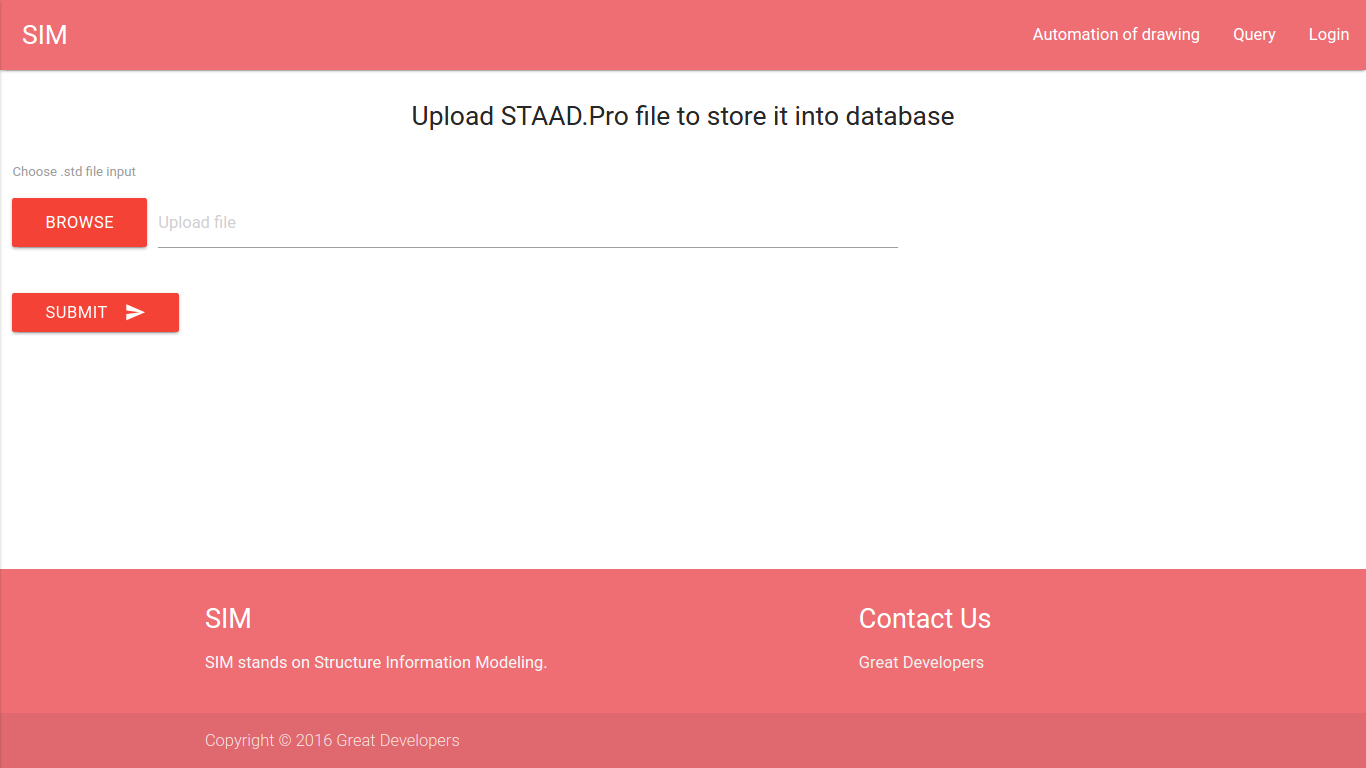
\includegraphics[scale=0.33]{images/sim_index.png}
\caption{Front page}
\end{center}
\end{figure}

If the system recognizes that the file in consideration is not correct then it must point that out to the user and also be able to tell that in what manner is the file wrong. For example, if the file is wrong syntactically then the correct syntactic suggestion must be provided to the user.  If the file is not complete then simply a message must be passed to the user.

\begin{figure}[h!]
\begin{center}
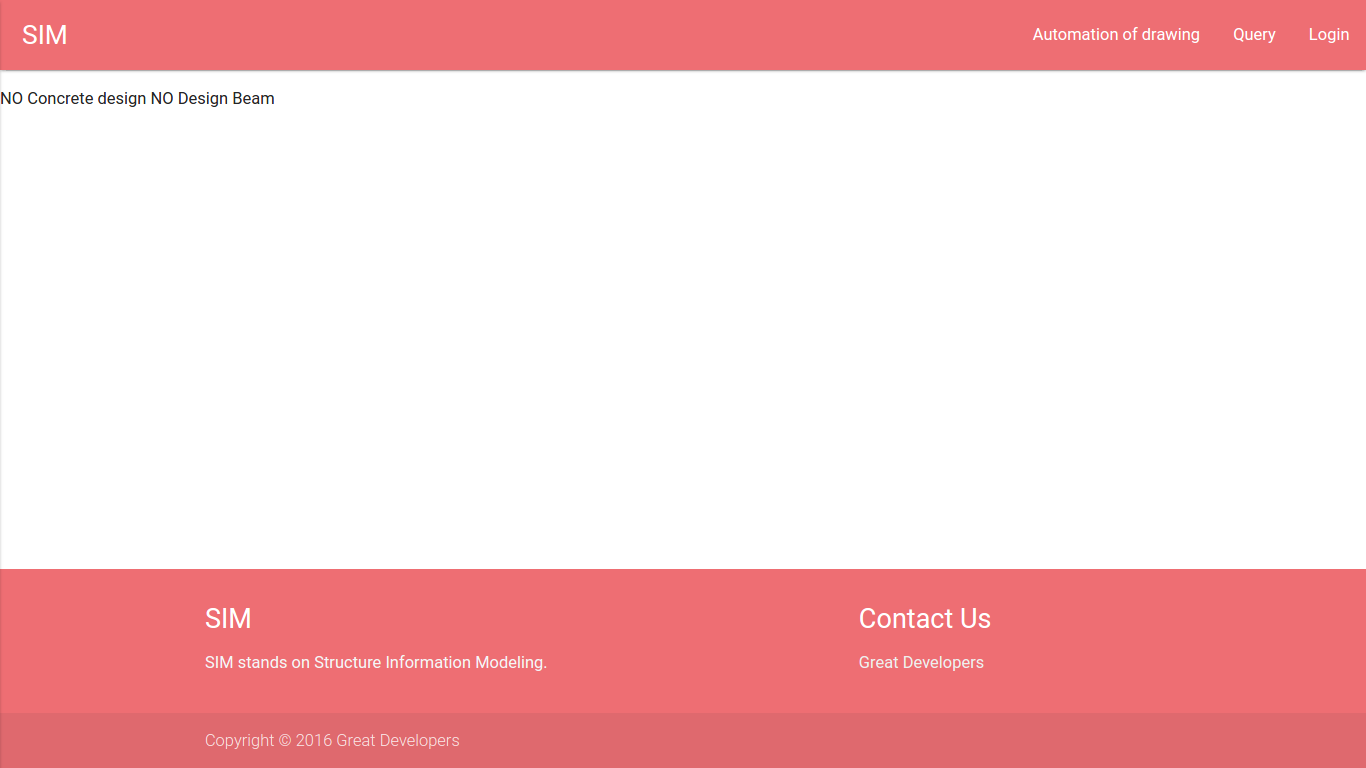
\includegraphics[scale=0.33]{images/after_upload.png}
\caption{Result show on submitted the Staad.Pro file}
\end{center}
\end{figure}
\newpage
\subsection{Query}
The user must be able to apply queries on the information stored in the databases.
All the data stored in the database is shown in the tabular form with all the fields that are related to the respective element as shown in Fig. 3.3.

\begin{figure}[h!]
\begin{center}
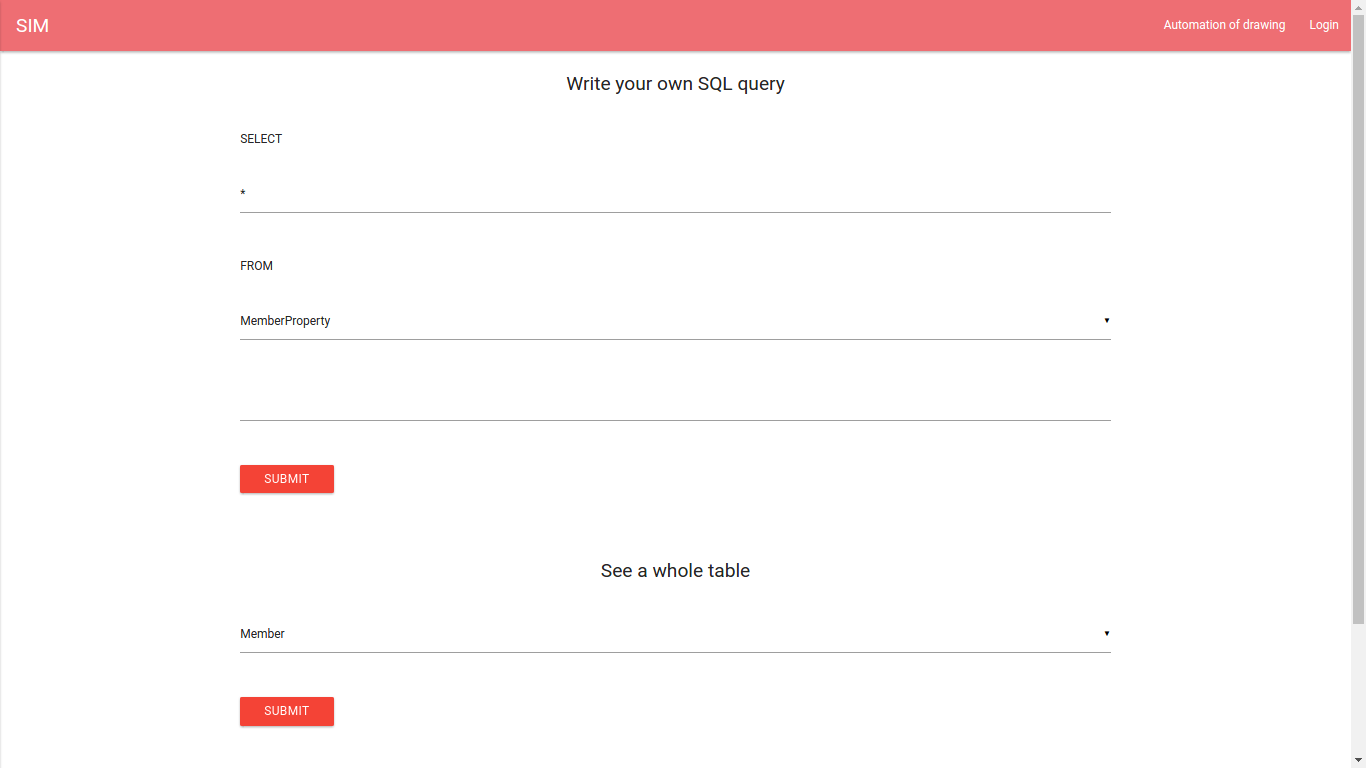
\includegraphics[scale=0.33]{images/query.png}
\caption{Query page}
\end{center}
\end{figure}

Result of the query is shown Fig. 3.4.

\begin{figure}[h!]
\begin{center}
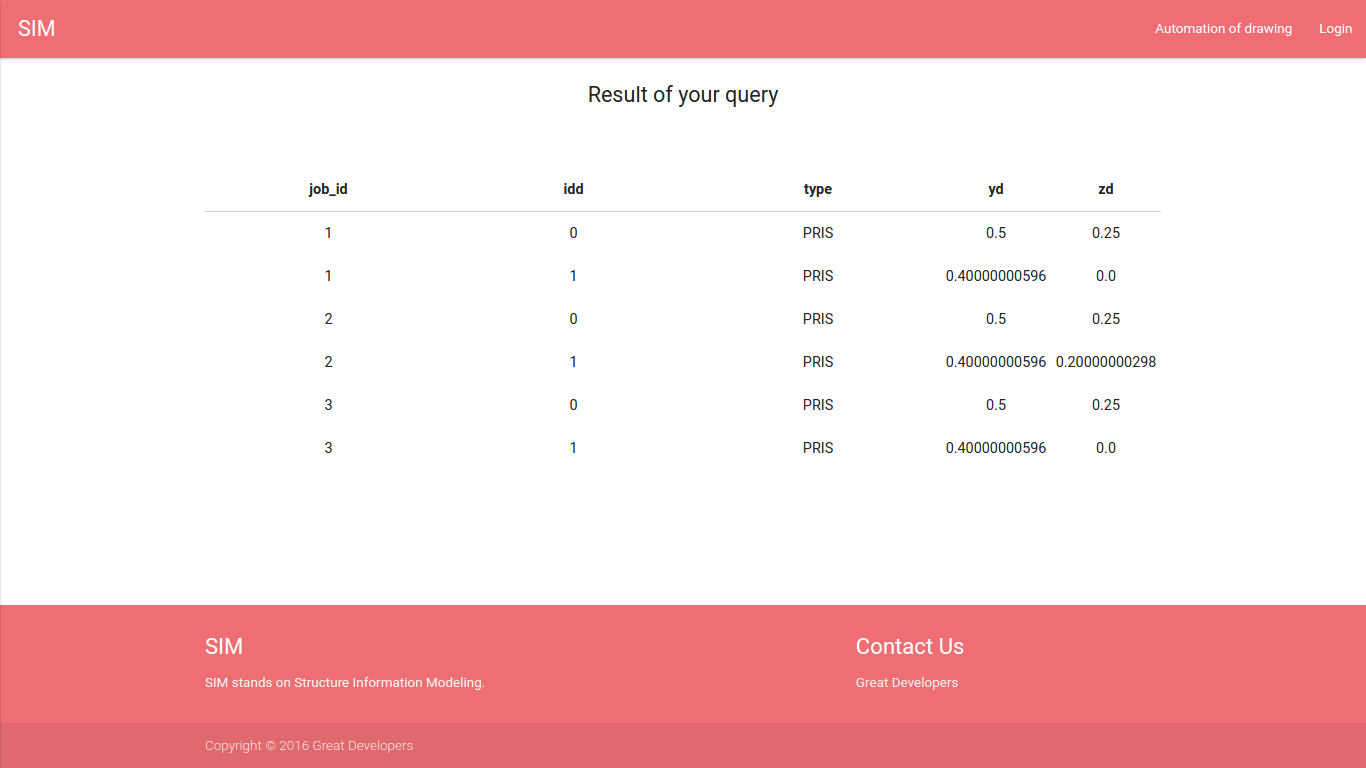
\includegraphics[scale=0.33]{images/result_query.png}
\caption{Result of query}
\end{center}
\end{figure}

\subsection{Automation of Drawings}
\subsubsection{Enter Building specifications}
The user makes the drawings of different views of the building on the
drawing sheets. The user will be able to enter the specifications of the building through the web
browser (Fig. 3.5) and on the back-end, the FreeCAD macros will use those input values to draw the drawings of different views of the building on different drawing
sheets. The output of the same can then be taken by a user in SVG, PDF and fcstd formats.

\begin{figure}[h!]
\begin{center}
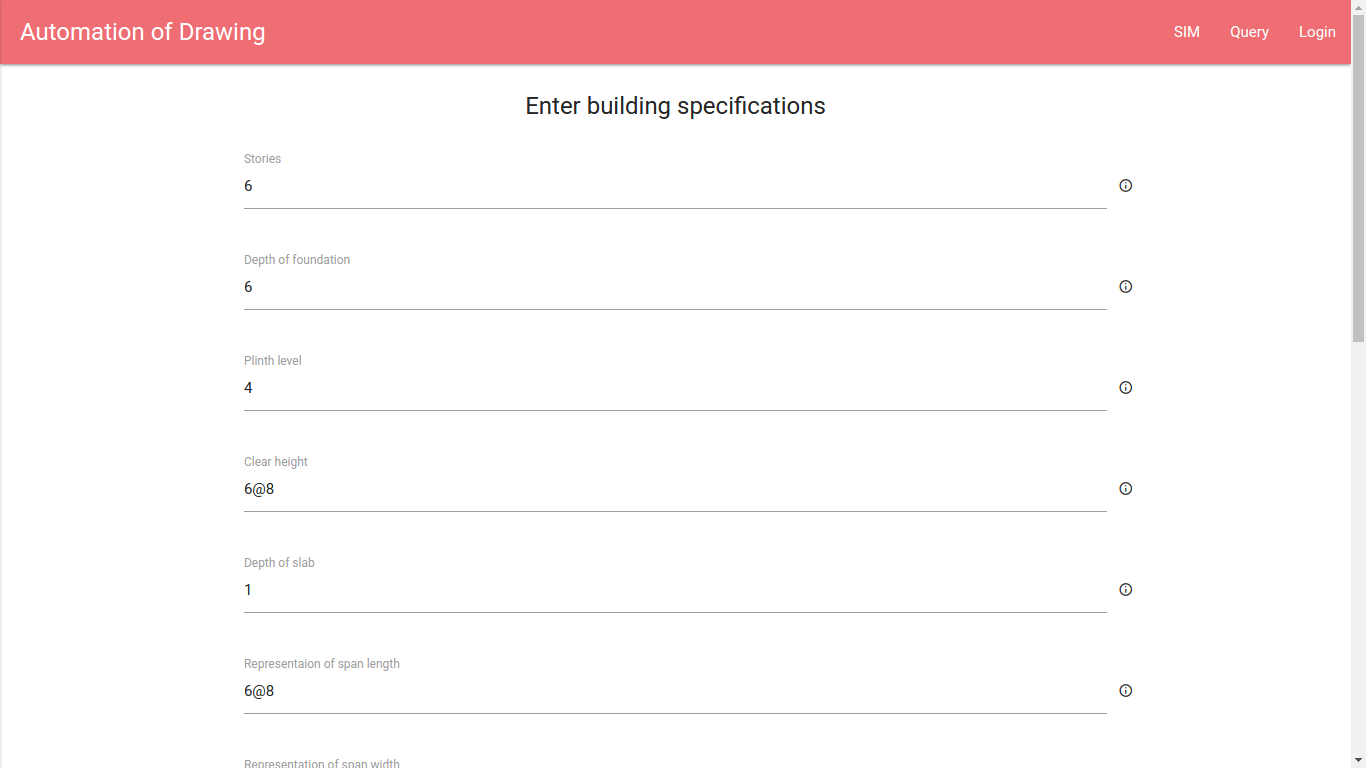
\includegraphics[scale=0.35]{images/auto_drawing.png}
\caption{Form to enter the specifications of the building}
\end{center}
\end{figure}

\subsubsection{Download project as zip}
After submitting the form this page will redirect to download page(Fig. 3.6). Here the user will see all the submitted value of in form (Fig. 3.5) and download its project.
\begin{figure}[h!]
\begin{center}
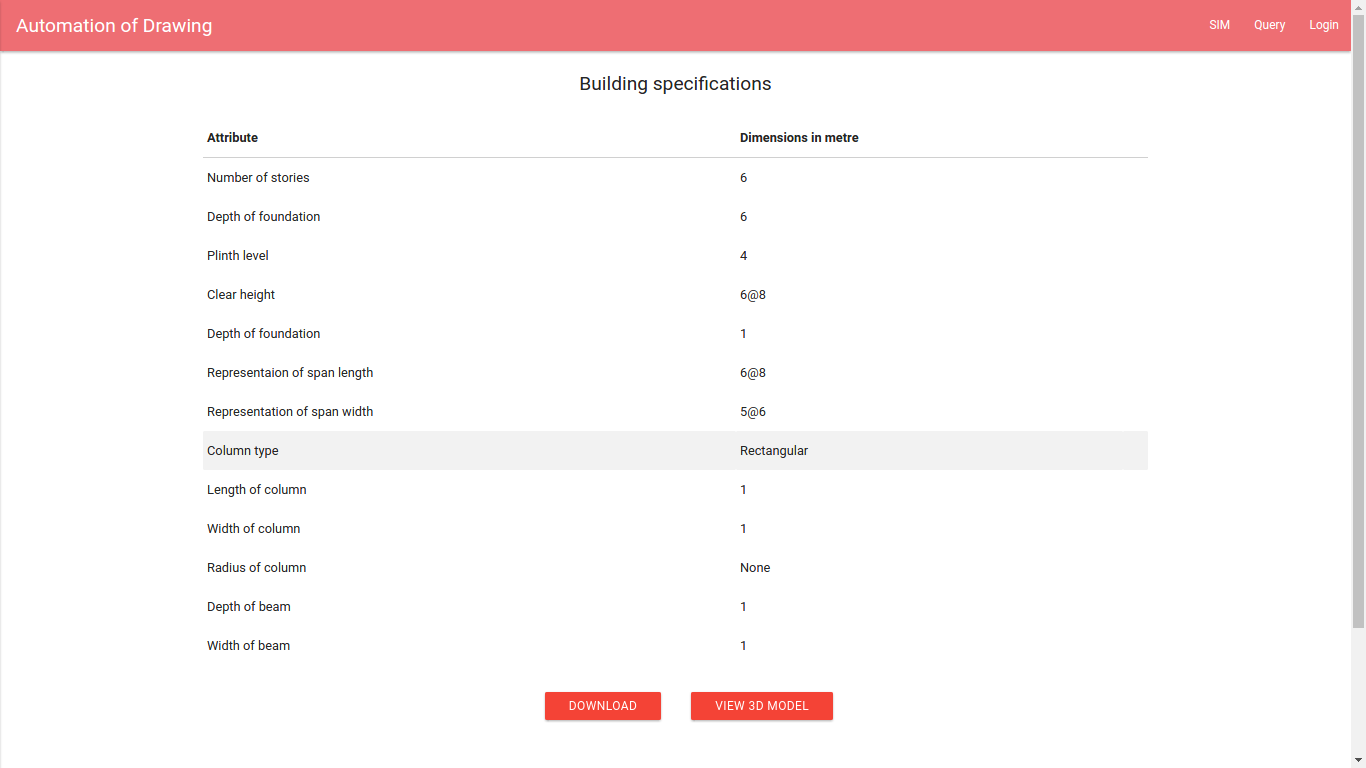
\includegraphics[scale=0.35]{images/b_specs.png}
\caption{Form to enter the specifications of the building}
\end{center}
\end{figure}
The zip file will contain different views (like side view, front view, a top view and many sectional views according to the building stories) of the building in PDF as well in SVG format. It also contains .fcstd file (FreeCAD project file) Fig. 3.7. By using .fcstd file the user will modify the existing project and can perform a wide range of operations.

\begin{figure}[h!]
\begin{center}
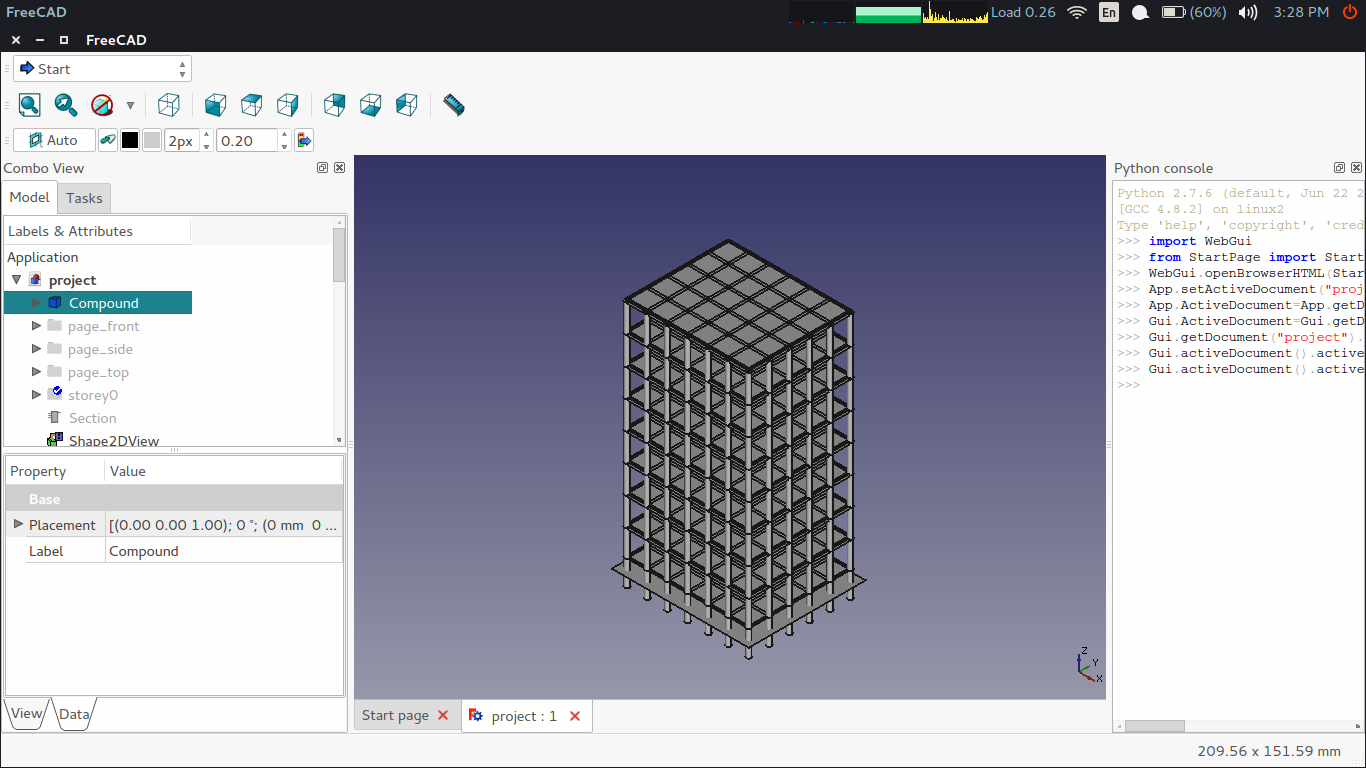
\includegraphics[scale=0.35]{images/building_macro.png}
\caption{Opening .fcstd file in FreeCAD}
\end{center}
\end{figure}

\subsubsection{View 3D model}
This feature will render the 3D model of the building on the browser screen. In this process, FreeCAD exporter convert .fcstd file to WebGL format (Web Graphics Library is a JavaScript API for rendering interactive 3D and 2D graphics within any compatible web browser without the use of plug-ins).   

\begin{figure}[h!]                                                      
\begin{center}                                                          
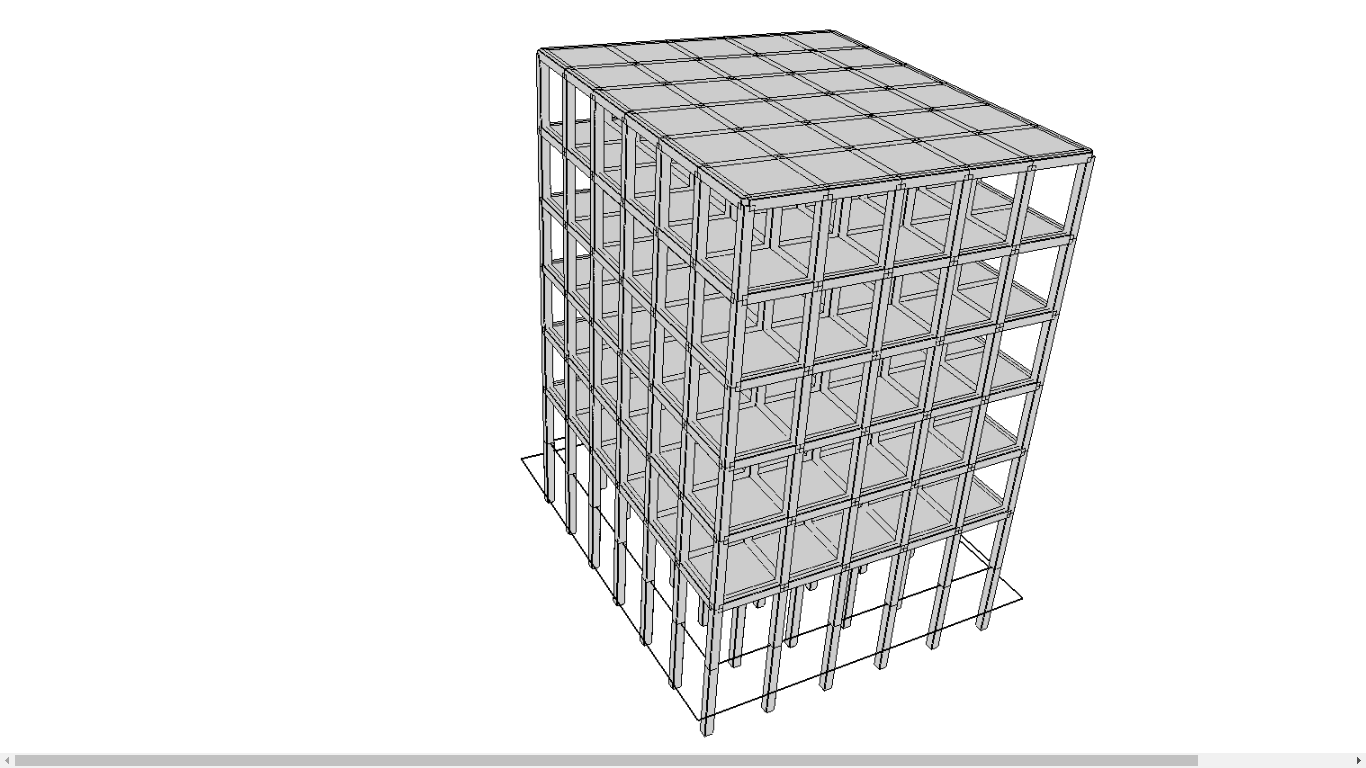
\includegraphics[scale=0.35]{images/3dmodel.png}                        
\caption{Admin page}              
\end{center}                                                            
\end{figure} 

\section{Adminstration Login}
One of the most powerful parts of SIM is the admin interface Fig . It reads metadata from your models to provide a quick, model-centric interface where trusted users can manage content on your site. The admin’s recommended use is limited to an organisation’s internal management tool. It’s not intended for building your entire front end around.

\begin{figure}[h!]                                                      
\begin{center}                                                          
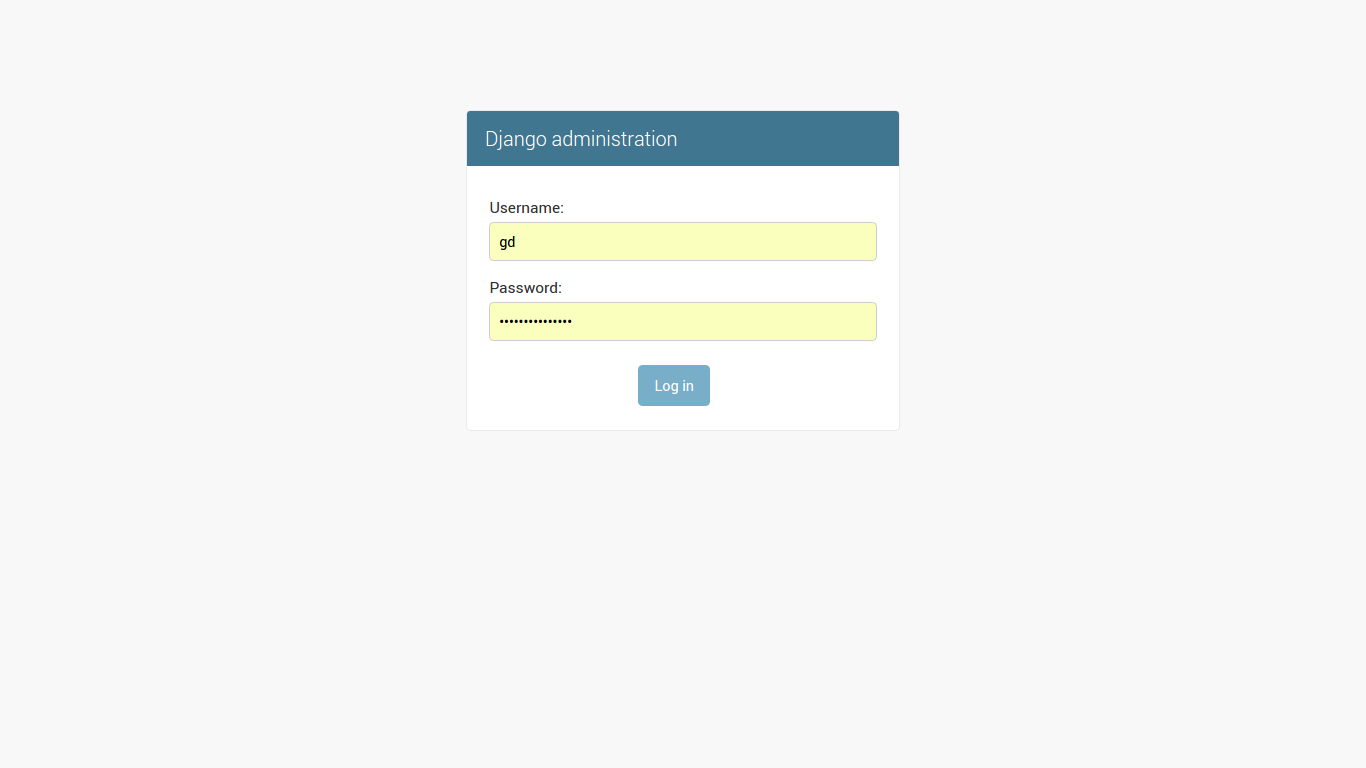
\includegraphics[scale=0.35]{images/admin.png}                        
\caption{Login page}                            
\end{center}                                                            
\end{figure} 

The admin has many hooks for customization, but beware of trying to use those hooks exclusively. If you need to provide a more process-centric interface that abstracts away the implementation details of database tables and fields, then it’s probably time to write your own views.

\begin{figure}[h!]                                                      
\begin{center}                                                          
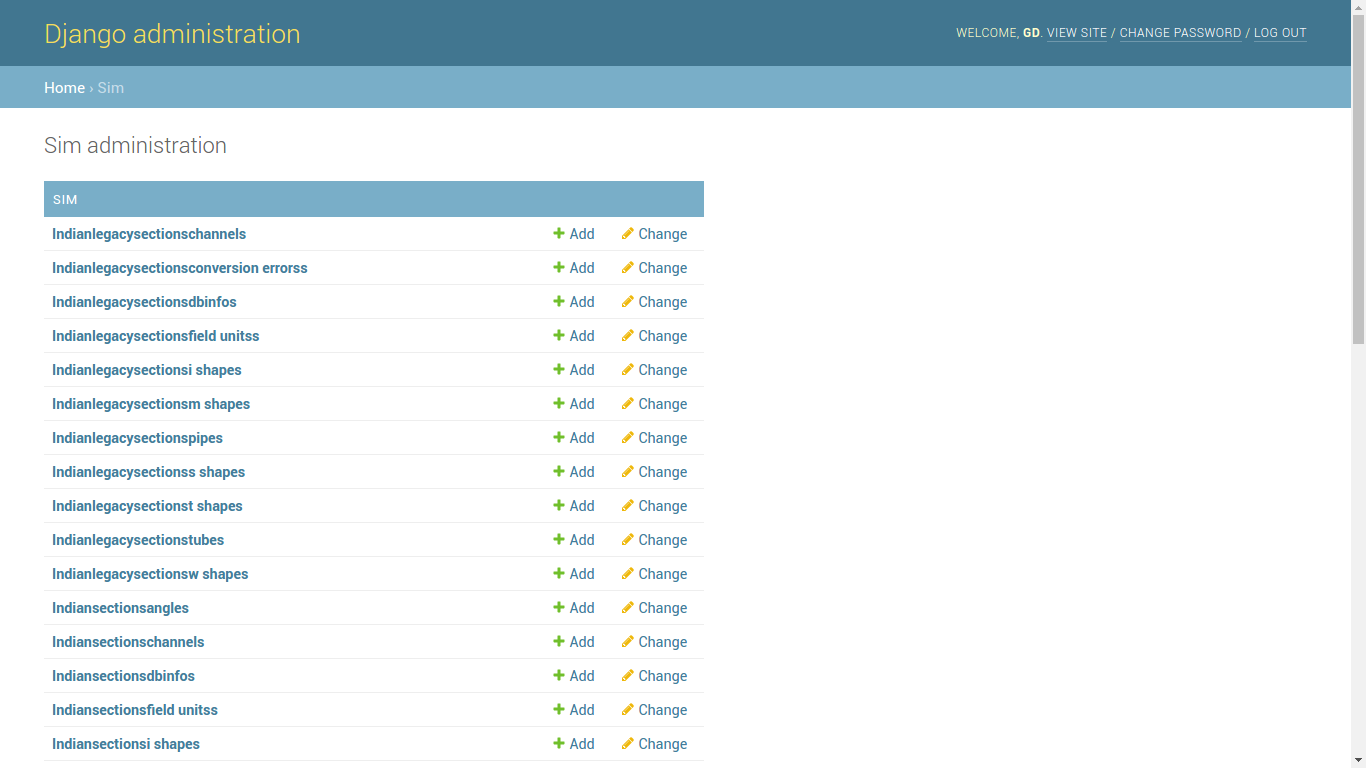
\includegraphics[scale=0.35]{images/admin2.png}                        
\caption{Entities of Staad Pro}                            
\end{center}                                                            
\end{figure} 

\begin{figure}[h!]                                                      
\begin{center}                                                          
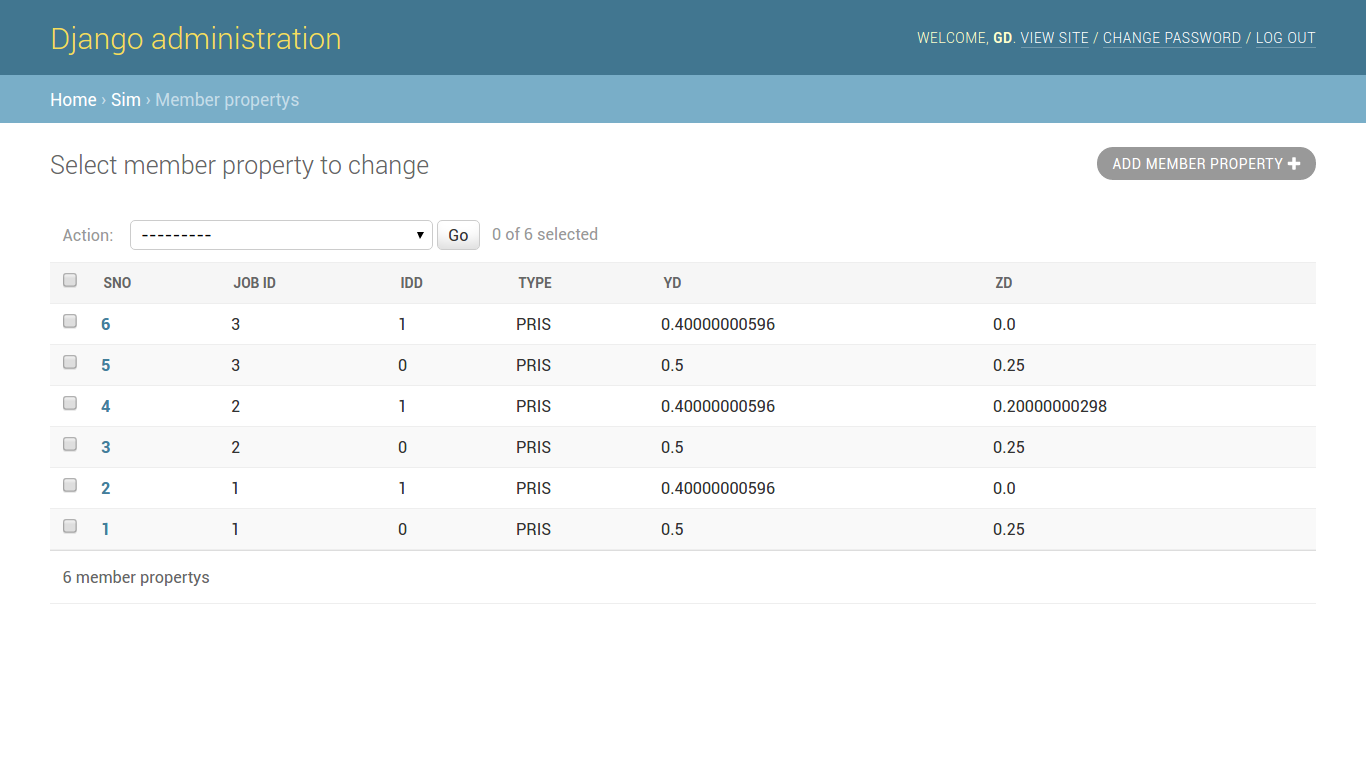
\includegraphics[scale=0.35]{images/admin3.png}                        
\caption{Attributes of each entity}                            
\end{center}                                                            
\end{figure} 

\begin{figure}[h!]                                                      
\begin{center}                                                          
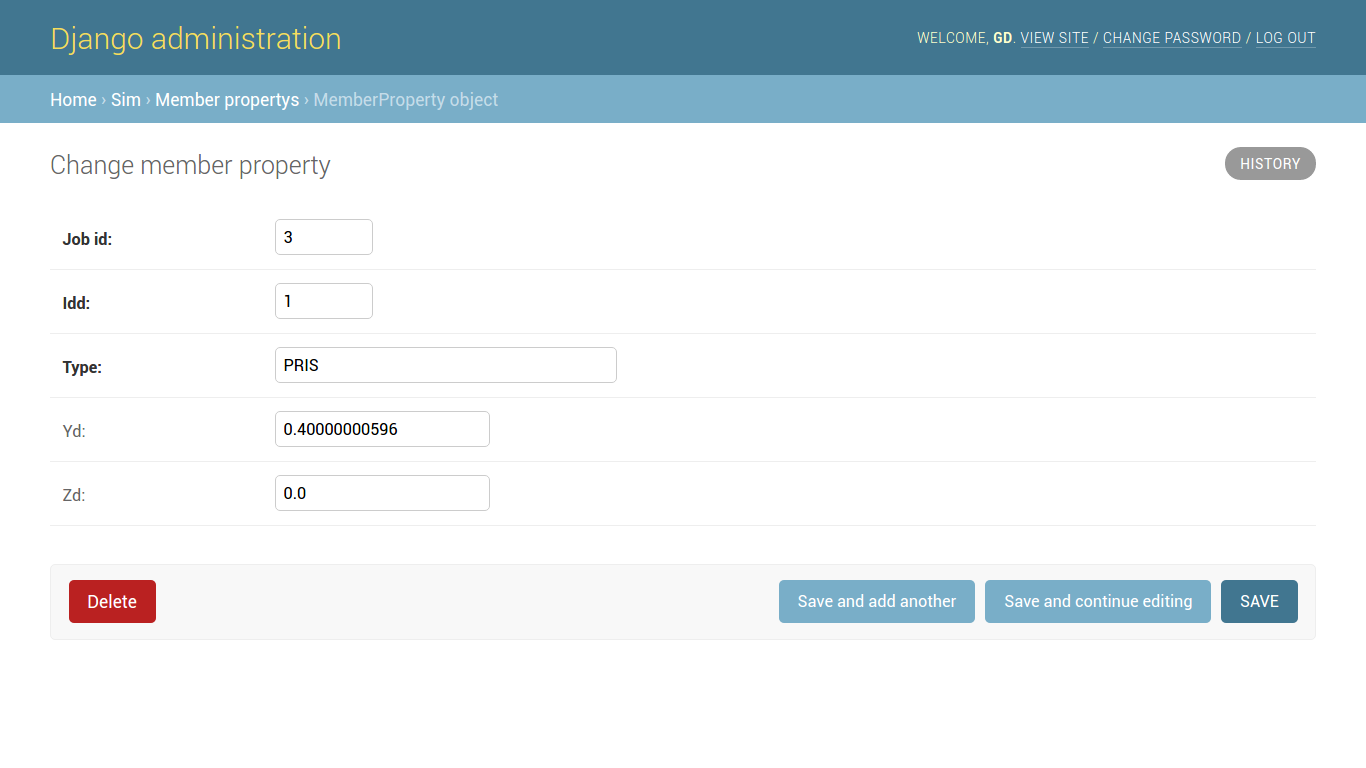
\includegraphics[scale=0.35]{images/admin4.png}                        
\caption{Modification, creation and deleting entity}                            
\end{center}                                                            
\end{figure} 

\end{comment}
